\documentclass[a4paper]{article}
\usepackage[utf8]{inputenc} % Skal passe til editorens indstillinger
\usepackage[english]{babel} % danske overskrifter


\newcommand{\name}{Carsten Nielsen}
%\newcommand{\stnumber}{s123369, s123161, s123821}
\newcommand{\course}{INI 404 Neuromorphic Engineering~I}
\newcommand{\university}{University of Zürich}
\newcommand{\studyline}{Institute of Neuroinformatics}
\newcommand{\assignment}{Lab 8 Post-Lab}
\renewcommand{\date}{\today} %If another date, than that of today is desiered


% Palatino for rm and math | Helvetica for ss | Courier for tt
\usepackage{mathpazo} % math & rm
\linespread{1.05}        % Palatino needs more leading (space between lines)
\usepackage{palatino} % tt
\normalfont
\usepackage[T1]{fontenc}
\usepackage[english]{babel}

\usepackage{graphicx}%allerese hentet % indsættelse af billeder
\usepackage{epstopdf} %Tilfj "--enable-write18" i argumentet for LaTex build. Dette vil konvertere .eps figurer til pdf-format
\graphicspath{{./picture/}} % stivej til bibliotek med figurer
\usepackage{subcaption} %Til gruppering af figurer
\usepackage{amsmath} %matpakke
\usepackage{amsfonts} %
\usepackage{amssymb} %
\usepackage{steinmetz} % flere matematik symboler
\usepackage{polynom} %for displaying polynom division
\usepackage{mathtools} % matematik - understøtter muligheden for at bruge \eqref{}
\usepackage{float}
\usepackage{placeins}
\usepackage{hhline}

%
\usepackage[usenames,dvipsnames]{xcolor}
\usepackage[compact,explicit]{titlesec}% http://ctan.org/pkg/titlesec
%
\usepackage[europeanresistors]{circuitikz}
\usepackage{pgfplots}
\usepgfplotslibrary{patchplots}
\pgfplotsset{compat=1.11}

%---------%
%Easy edit%
%---------%

%Section formating. arg1 is supplied when making section
\newcommand\presectionnumber[1]{~~}
\newcommand\postsectionnumber[1]{}
\newcommand\midlesection[1]{#1}
\newcommand\sectionnum[1]{\arabic{#1}}
\newcommand\subsectionnum[1]{\arabic{#1}}
\newcommand\subsubsectionnum[1]{\alph{#1}}



%------------%
%setion setup%
%------------%
\renewcommand\thesection{Opgave~\sectionnum{section}} %pas p�, kun i matematik
\renewcommand\thesubsection{\thesection,~\subsectionnum{subsection}}
\definecolor{MagRed}{RGB}{190,40,15}
\definecolor{MathGreen}{RGB}{82,164,0}

\titleformat{\section}{\normalfont\sffamily\large\bfseries\color{MathGreen}}{}{0pt}{|\kern-0.15ex|\kern-0.15ex|\kern-0.15ex|\presectionnumber{#1}\sectionnum{section}\postsectionnumber{#1}\qquad\quad\midlesection{#1}\label{sec:\sectionnum{section}}}
\titleformat{\subsection}[runin]{\large\bfseries}{}{10pt}{\sectionnum{section}.\subsectionnum{subsection})~#1\label{sec:\sectionnum{section}.\subsectionnum{subsection}}}
\titleformat{\subsubsection}[runin]{\itshape}{}{0pt}{\subsectionnum{subsection},\subsubsectionnum{subsection}~#1\label{sec:\sectionnum{section}.\subsectionnum{subsection}.\subsubsectionnum{subsubsection}}}
%\titleformat{\subsubsection}{\bfseries}{}{0pt}{\alph{subsection}.\arabic{subsubsection})\qquad\quad#1\label{\arabic{section}\alph{subsection}\arabic{subsubsection}}}

%----------%
%page setup%
%----------%
\textwidth = 400pt
\marginparwidth = 86pt
\hoffset = -25pt
\voffset= -30pt
\textheight = 670pt

%--------%
%hyperref%
%--------%
\newcommand{\HRule}{\rule{\linewidth}{0.5mm}}
\usepackage{fancyhdr}
\usepackage[plainpages=false,pdfpagelabels,pageanchor=false]{hyperref} % aktive links
\hypersetup{%
  pdfauthor={\name},
  pdftitle={\assignment},
  pdfsubject={\course} }
%\usepackage{memhfixc}% rettelser til hyperref

%-------------%
%Headder setup%
%-------------%
\fancyhf{} % tom header/footer
\fancyhfoffset{20pt}
\fancyhfoffset{20pt}
\fancyhead[OL]{\name \\ INI 404}
\fancyhead[OC]{Date \\ \date}
\fancyhead[OR]{\university\\ \studyline}
\fancyfoot[FL]{}
\fancyfoot[FC]{\thepage}
\fancyfoot[FR]{}
\renewcommand{\headrulewidth}{0.4pt}
\renewcommand{\footrulewidth}{0.4pt}
\headsep = 35pt
\pagestyle{fancy}
 % style setup

%Listings%
\usepackage{listingsutf8}
\usepackage[framed,numbered]{matlab-prettifier}


%setup listings
\lstset{language=Matlab,
  extendedchars=true,
  language=Octave,                % the language of the code
  basicstyle=\ttfamily\footnotesize,           % the size of the fonts that are
  % used for the code
  numbers=left,                   % where to put the line-numbers
  numberstyle=\tiny\color{gray},  % the style that is used for the line-numbers
  stepnumber=2,                   % the step between two line-numbers. If it's 1, each line 
                                  % will be numbered
  numbersep=5pt,                  % how far the line-numbers are from the code
  backgroundcolor=\color{white},      % choose the background color. You must add \usepackage{color}
  showspaces=false,               % show spaces adding particular underscores
  showstringspaces=false,         % underline spaces within strings
  showtabs=false,                 % show tabs within strings adding particular underscores
  frame=single,                   % adds a frame around the code
  rulecolor=\color{black},        % if not set, the frame-color may be changed on line-breaks within not-black text (e.g. comments (green here))
  tabsize=4,                      % sets default tabsize to 2 spaces
  captionpos=b,                   % sets the caption-position to bottom
  breaklines=true,                % sets automatic line breaking
  breakatwhitespace=false,        % sets if automatic breaks should only happen at whitespace
  title=\lstname,                   % show the filename of files included with \lstinputlisting;
                                  % also try caption instead of title
  %keywordstyle=\color{blue},          % keyword style
  %commentstyle=\color{dkgreen},       % comment style
  %stringstyle=\color{mauve},         % string literal style
  escapeinside={\%*}{*)},            % if you want to add LaTeX within your code
  morekeywords={*,...},              % if you want to add more keywords to the set
  deletekeywords={...}              % if you want to delete keywords from the given language
}
\lstset{literate=
  {á}{{\'a}}1 {é}{{\'e}}1 {í}{{\'i}}1 {ó}{{\'o}}1 {ú}{{\'u}}1
  {Á}{{\'A}}1 {É}{{\'E}}1 {Í}{{\'I}}1 {Ó}{{\'O}}1 {Ú}{{\'U}}1
  {à}{{\`a}}1 {è}{{\`e}}1 {ì}{{\`i}}1 {ò}{{\`o}}1 {ù}{{\`u}}1
  {À}{{\`A}}1 {È}{{\'E}}1 {Ì}{{\`I}}1 {Ò}{{\`O}}1 {Ù}{{\`U}}1
  {ä}{{\"a}}1 {ë}{{\"e}}1 {ï}{{\"i}}1 {ö}{{\"o}}1 {ü}{{\"u}}1
  {Ä}{{\"A}}1 {Ë}{{\"E}}1 {Ï}{{\"I}}1 {Ö}{{\"O}}1 {Ü}{{\"U}}1
  {â}{{\^a}}1 {ê}{{\^e}}1 {î}{{\^i}}1 {ô}{{\^o}}1 {û}{{\^u}}1
  {Â}{{\^A}}1 {Ê}{{\^E}}1 {Î}{{\^I}}1 {Ô}{{\^O}}1 {Û}{{\^U}}1
  {œ}{{\oe}}1 {Œ}{{\OE}}1 {æ}{{\ae}}1 {Æ}{{\AE}}1 {ß}{{\ss}}1
  {ç}{{\c c}}1 {Ç}{{\c C}}1 {ø}{{\o}}1 {å}{{\r a}}1 {Å}{{\r A}}1
  {€}{{\EUR}}1 {£}{{\pounds}}1
}

 \lstloadlanguages{% Check Dokumentation for further languages ...
         %[Visual]Basic
         %Pascal
         %C
         %C++
         %XML
         %HTML
         %Java
         %VHDL
         Matlab
 }
 %Listings slut%









%Matematik hurtige ting
%fed
\renewcommand\vec[1]{\mathbf{#1}}
\newcommand\matr[3]{{}_{#2}\mathbf{#1}{}_{#3}}
\newcommand\facit[1]{\underline{\underline{#1}}}
%\renewcommand\d[3]{\frac{\mbox{d}^{#3}#1(#2)}{\mbox{d}#2^{#3}}}
%underline
%\renewcommand\vec[1]{\underline{#1}}
%\newcommand\matr[3]{{}_{#2}\underline{\underline{#1}}{}_{#3}}

\renewcommand\matrix[4]{ %{alignment}{to space}{from space}{matrix}
{\vphantom{\left[\begin{array}{#1}#4\end{array}\right]}}_{#2}\kern-0.5ex
\left[\begin{array}{#1}
#4
\end{array}\right]_{#3}
}
\newcommand\e[0]{\mbox{e}}
\newcommand\E[1]{\cdot 10^{#1}}
\newcommand\im[0]{i}

\newcommand\Jaco{\mbox{Jacobi}}
\newcommand\del[2]{\frac{\partial {#1}}{\partial {#2}}}
\newcommand\abs[1]{\left| {#1} \right|}
\newcommand\stdfig[4]{ %width,img,cap,lab
\begin{figure}[H]
\centering
\includegraphics[width={#1}\textwidth]{#2}
\caption{#3}
\label{#4}
\end{figure}
}
\newcommand\stdfignoscale[3]{ %img,cap,lab
\begin{figure}[H]
\centering
\includegraphics{#1}
\caption{#2}
\label{#3}
\end{figure}
}
\newcommand\diff{\dot}
\newcommand\ddiff{\ddot}
\newcommand\dddiff{\dddot}
\newcommand\ddddiff{\ddddot}






% How to make ref to books or urls in bib
%\citetitle[fx: page 1]{name of ref in bib}


\tikzset{rrail/.style={rground,yscale=-1}}
\newcommand{\reffig}[1]{Fig.~\ref{#1}}

\begin{document}
\begin{titlepage}
\centering \parindent=0pt

\vspace*{\stretch{1}} \HRule\\[1cm]\Huge
\course\\[0.7cm]
\large \assignment\\[1cm]
\HRule\\[4cm]  
%\includegraphics[width=6cm]{picture}\\ Use this if you want a picture on the frontpage
\name\\
%\stnumber
TAs: Ning Quiao, Chenghan Li

\vspace*{\stretch{2}} \normalsize %

\begin{center}
	\date 
\end{center}
\vspace*{\stretch{2}} \normalsize
\begin{flushright}
%\includegraphics[width=6cm]{./dtu.eps}\\
\end{flushright}
\end{titlepage}

\newpage

In this lab we test a non-volatile analog memory cell. The cell stores charge in an isolated 'floating' gate using quantum tunneling and hot electron injection. 

The chips that were  available to us did not seem to work properly so we are using the data obtained by the group of M. Milde et al. for this report. \\

\section{Measuring Injection and Tunneling Current}

Here we show examples of injection and tunneling and demonstrate how to calculate the currents that flow into the floating gate. 

In Fig.~\ref{fig:exp1a} we can see how the output voltage of the circuit increases linearly as we inject electrons into the floating gate. The injection current can be calculated as follows:

\begin{equation*}
	V_{out}\approx V_{inp}+V_c
\end{equation*}

\begin{equation*}
	\frac{dV_{out}}{dt}\approx \frac{dV_c}{dt} = \frac{I_{inj}}{C}
\end{equation*}
So that
\begin{equation*}
	I_{inj} = C\frac{dV_{out}}{dt}
\end{equation*}
In the case of Fig.~\ref{fig:exp1a}, the injection current will therefore be 
\begin{equation*}
	I_{inj}=2\cdot10^{-12}\cdot0.0714 = 1.43\cdot10^{-13} A\\
\end{equation*}

\begin{figure}[!h]
	\center
	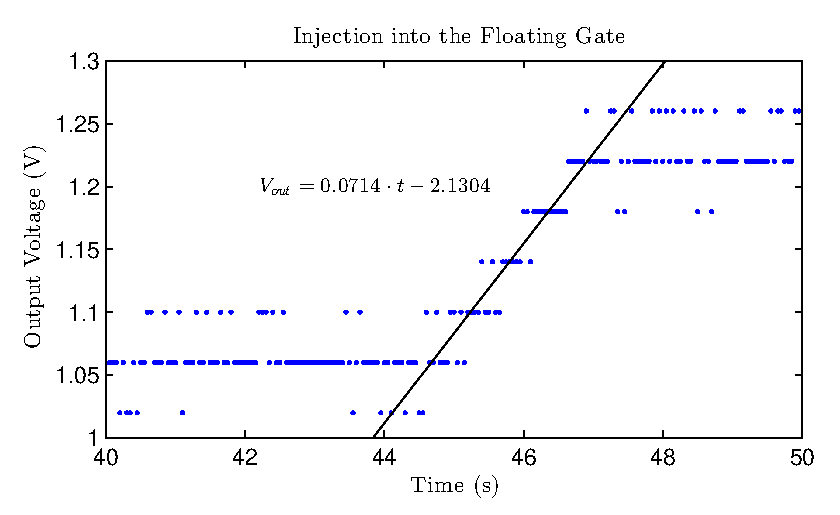
\includegraphics{exp1a.eps}
	\caption{Output voltage of the circuit as we inject electrons into the floating gate with $V_{inj}=5 V$. The line corresponds to a linear fit.}
	\label{fig:exp1a}
\end{figure}

Fig.~\ref{fig:exp1b} shows the output of the circuit as we perform tunneling. Similarly, the tunneling current can be calculated as

\begin{equation*}
	I_{tun} = -C\frac{dV_{out}}{dt}
\end{equation*}

So we obtain 
\begin{equation*}
	I_{inj}=-2\cdot10^{-12}\cdot(-0.1682) = 3.36\cdot10^{-13} A\\
\end{equation*}

\begin{figure}[!h]
	\center
	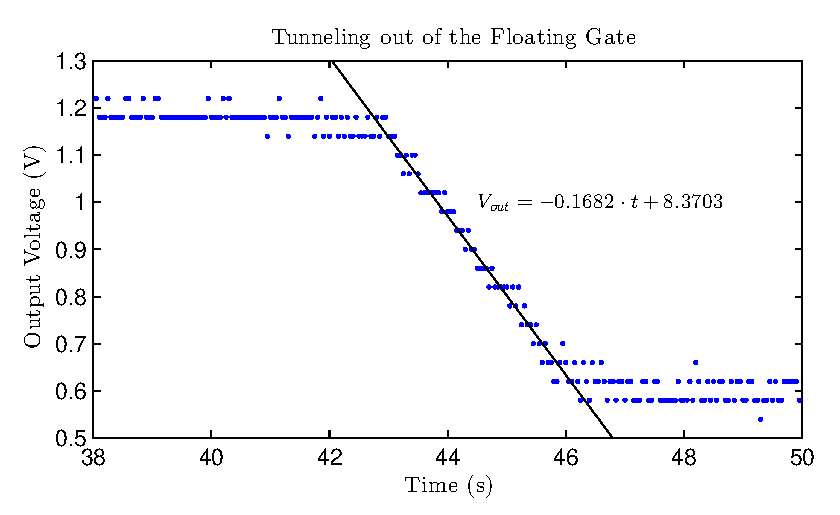
\includegraphics{exp1b.eps}
	\caption{Output voltage of the circuit as we tunnel electrons out of the floating gate and a linear fit.}
	\label{fig:exp1b}
\end{figure}

\section{pFET Injection}

In this experiment we measure the output voltage of the circuit for five different values of $V_{inj}$ between 10 V and 10.5 V and infer the injection currents as explained above. 

The efficiency of the injection (injection current divided by the current through the injection transistor) is plotted in Fig.~\ref{fig:exp2}.

\begin{figure}[!h]
	\center
	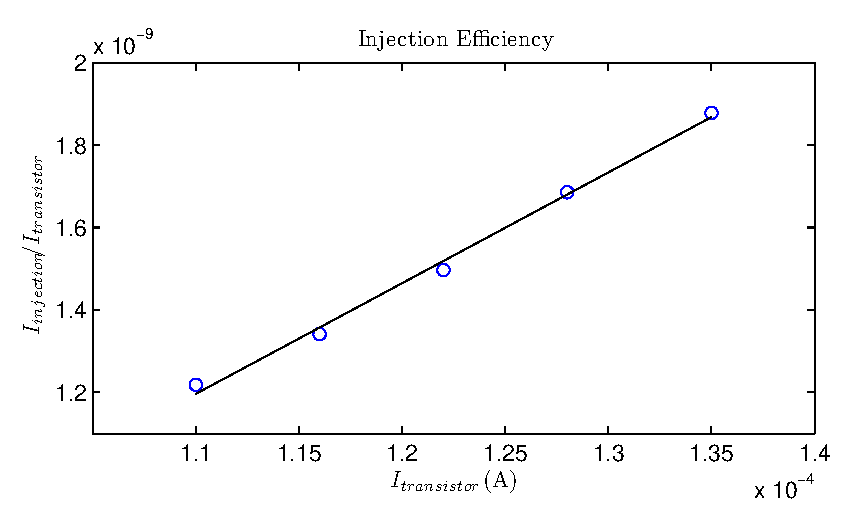
\includegraphics{exp2.eps}
	\caption{Injection efficiency ($I_{inj}/I_{transistor}$) as a function of the source current, $I_{transistor}$. The line represents the linear fit: $Efficiency = 2.6886\cdot10^{-5} I_{transistor} -2\cdot10^{-9}$.}
	\label{fig:exp2}
\end{figure}

The injection current can be characterized by 
\begin{equation*}
	I_{inj} = I_{transistor}~e^{\frac{V_{dc}}{V_{i}}}
\end{equation*}
where $V_i$ is a constant and $V_{dc}$ is the drain to channel voltage in the injection transistor. In this term, the drain voltage is constant (0 V) and the channel voltage is approximately constant. This is so because the channel voltage is related to the floating gate voltage, and this is kept close to $V_{inp}$ by the transconductance amplifier and the negative feedback. Therefore, it makes sense that the injection current is approximately proportional to the current through the transistor as we can see in Fig.~\ref{fig:exp2}.
\\
\section{Gate Oxide Tunneling}

Lastly, we compute the tunneling currents for five different values of $V_{tun}$ between 27 and 32 V. Figs.~\ref{fig:exp3a} and \ref{fig:exp3b} show the results. 
\begin{figure}[!h]
	\center
	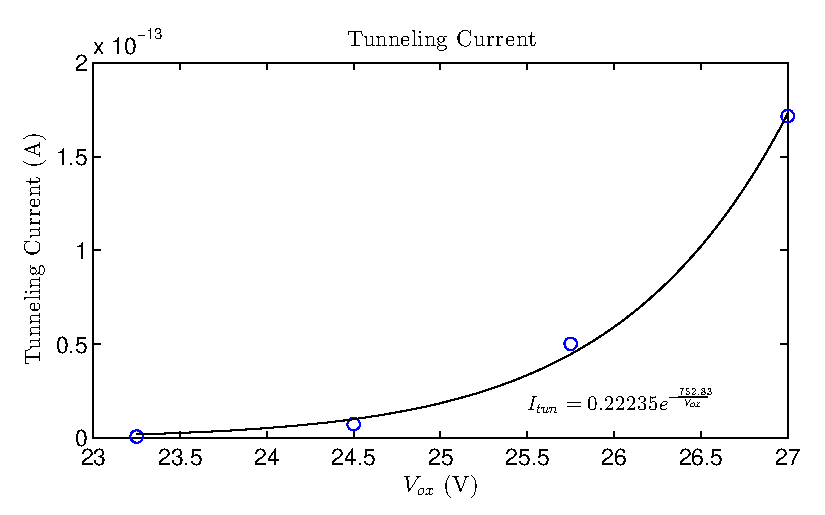
\includegraphics{exp3a.eps}
	\caption{Tunneling current as a function of the oxide voltage, $V_{ox}$ (i.e. $V_{tun}-V_{fg}$). $V_{fg}$ is assumed to be equal to $V_{inp}$. The curve represents a fit with a model of the form $I_{tun}=I_0e^{-\frac{V_0}{V_{ox}}}$.}
	\label{fig:exp3a}
\end{figure}


\begin{figure}[!h]
	\center
	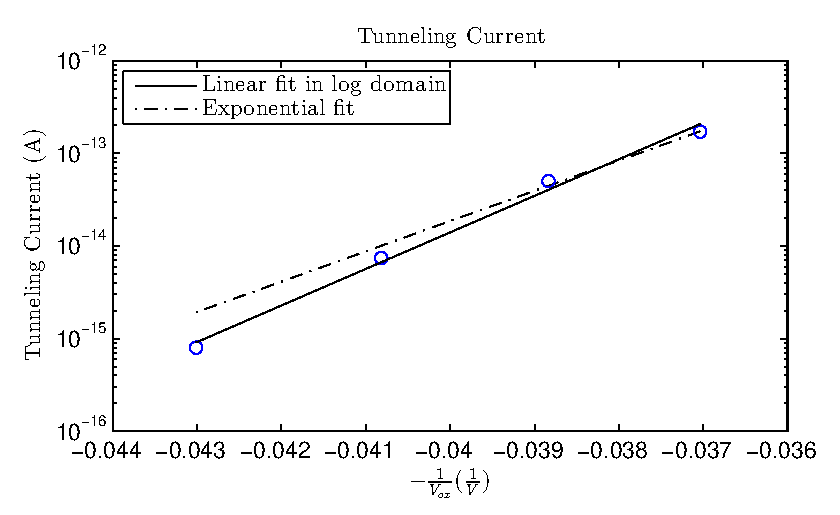
\includegraphics{exp3b.eps}
	\caption{Tunneling current in logarithmic scale, $log(I_{tun})$, as a function of $-1/V_{ox}$ and a linear fit (solid line). The dashed line corresponds to the exponential fit of Fig.~\ref{fig:exp3a}.}
	\label{fig:exp3b}
\end{figure}

The data has been fitted with a model of the form $I_{tun}=I_0e^{-\frac{V_0}{V_{ox}}}$. In this model, $I_0$ indicates value at which the tunneling current saturates and $V_{0}$ is a constant that depends on the thickness of the oxide. The thicker the oxide, the higher the oxide voltage that needs to be applied in order to get a certain current. 

In Fig.~\ref{fig:exp3a} the fit is done using the model directly and the original data. We obtain $I_0=0.22235$ A and $V_{0}=752.83$ V. In Fig.~\ref{fig:exp3b}, a line is fitted to the logarithm of the current as a function of $-1/V_{ox}$. With this we obtain $I_0=85.129$ A and $V_{0}=908.54$ V.

The model fits the data reasonably well. However, the points measured lie in the initial part of the equation that resembles a positive exponential, so we do not get to see the change in curvature and saturation of the current that the model predicts for higher voltages. 


\end{document}
